\documentclass[crop,tikz,border=5pt]{standalone}

\usetikzlibrary{fit,positioning,shapes.geometric,backgrounds,decorations.pathmorphing,decorations.markings,arrows.meta,shadows,decorations.pathreplacing}

\usepackage{libertine}          % Linux Libertine (serif)
\usepackage[libertine]{newtxmath} % Math fonts (compatible with Libertine)
\usepackage{inconsolata}        % Monospace
\usepackage[T1]{fontenc}        % Better font encoding
\usepackage{amsmath}            % Required for newtxmath

\begin{document}
  \def\pathid#1{\tikz[baseline]{\node[draw, thick, circle, anchor=base, font=\footnotesize] {#1};}}

  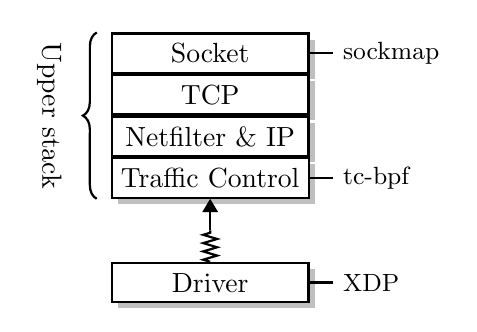
\begin{tikzpicture}[
    layer/.style={draw, thick, fill=white, drop shadow, minimum width=2.5cm, minimum height=0.5cm, align=center},
    backlog/.style={draw, thick, decorate, decoration={zigzag,segment length=3pt}},
    sidelabel/.style={rectangle, text width=2cm, text centered, minimum height=0.5cm, rotate=-90}
  ] 
    % Stack layers
    \node[layer, label={[font=\small, label distance=0.3cm]right:sockmap}] (socket) {Socket};
    \node[layer, anchor=north] at (socket.south) (tcp) {TCP};
    \node[layer, anchor=north] at (tcp.south) (netfilter) {Netfilter \& IP};
    \node[layer, anchor=north, label={[font=\small, label distance=0.3cm]right:tc-bpf}] at (netfilter.south) (tc) {Traffic Control};
    \node[layer, anchor=north, label={[font=\small, label distance=0.3cm]right:XDP}] at ([yshift=-0.8cm]tc.south) (driver) {Driver};

    \draw[decoration={brace,amplitude=5pt,raise=5pt},decorate, thick] (tc.south west) -- (socket.north west);
    \node[sidelabel, anchor=north] at ([xshift=-0.5cm]tcp.south west) {Upper stack};

    % Per-CPU backlog queue
    \draw[backlog] (driver.north) -- ([yshift=0.4cm]driver.north);
    \draw[thick, -Triangle] ([yshift=0.4cm]driver.north) -- (tc.south);

    % BPF Hooks
    \draw[thick] (socket.east) -- ([xshift=0.3cm]socket.east);
    \draw[thick] (tc.east) -- ([xshift=0.3cm]tc.east);
    \draw[thick] (driver.east) -- ([xshift=0.3cm]driver.east);
  \end{tikzpicture}
\end{document}

% convert -density 200 -quality 90 linux-networking-stack.{pdf,png}
